\begin{figure*}[!t]
  \centering
  \begin{subfigure}[b]{0.6\linewidth}
    \centering
    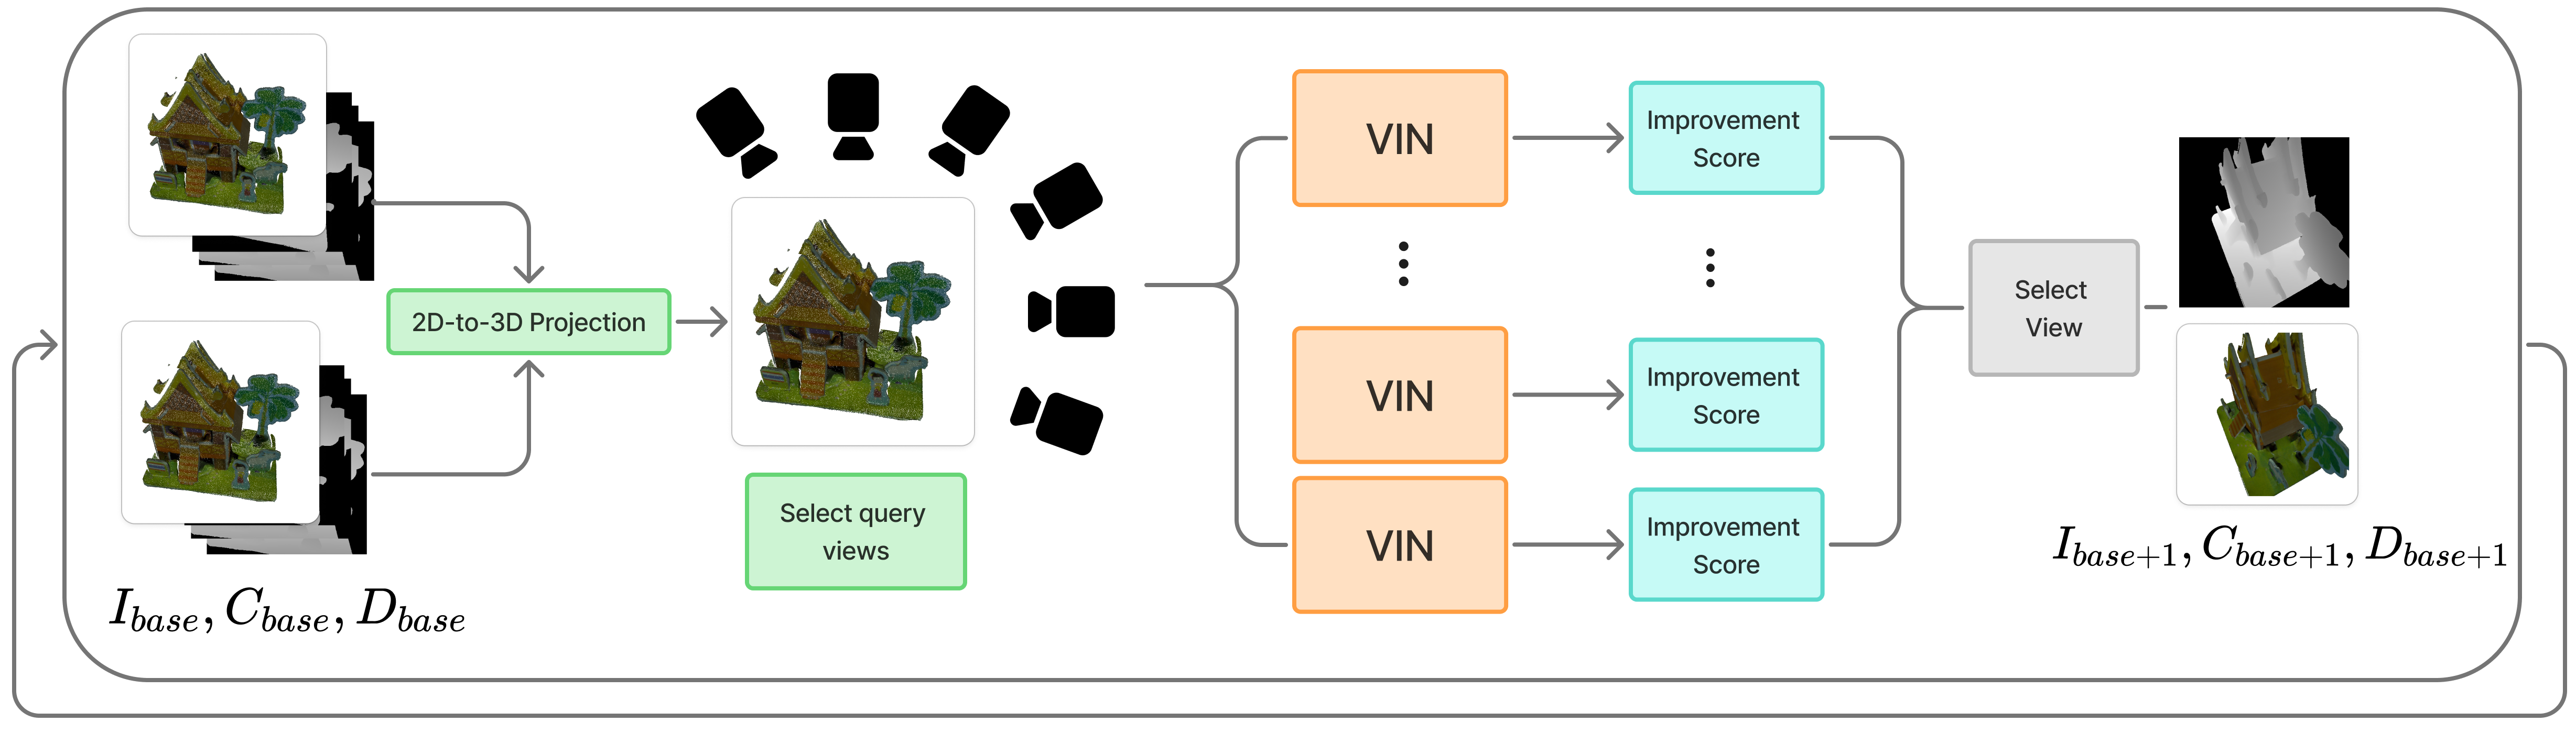
\includegraphics[width=\linewidth]{Figures/VIN-NBV_diagram.png}
    \caption{VIN-NBV Policy Overview}
    \label{fig:arch_left}
  \end{subfigure}
  \hfill
  \begin{subfigure}[b]{0.39\linewidth}
    \centering
    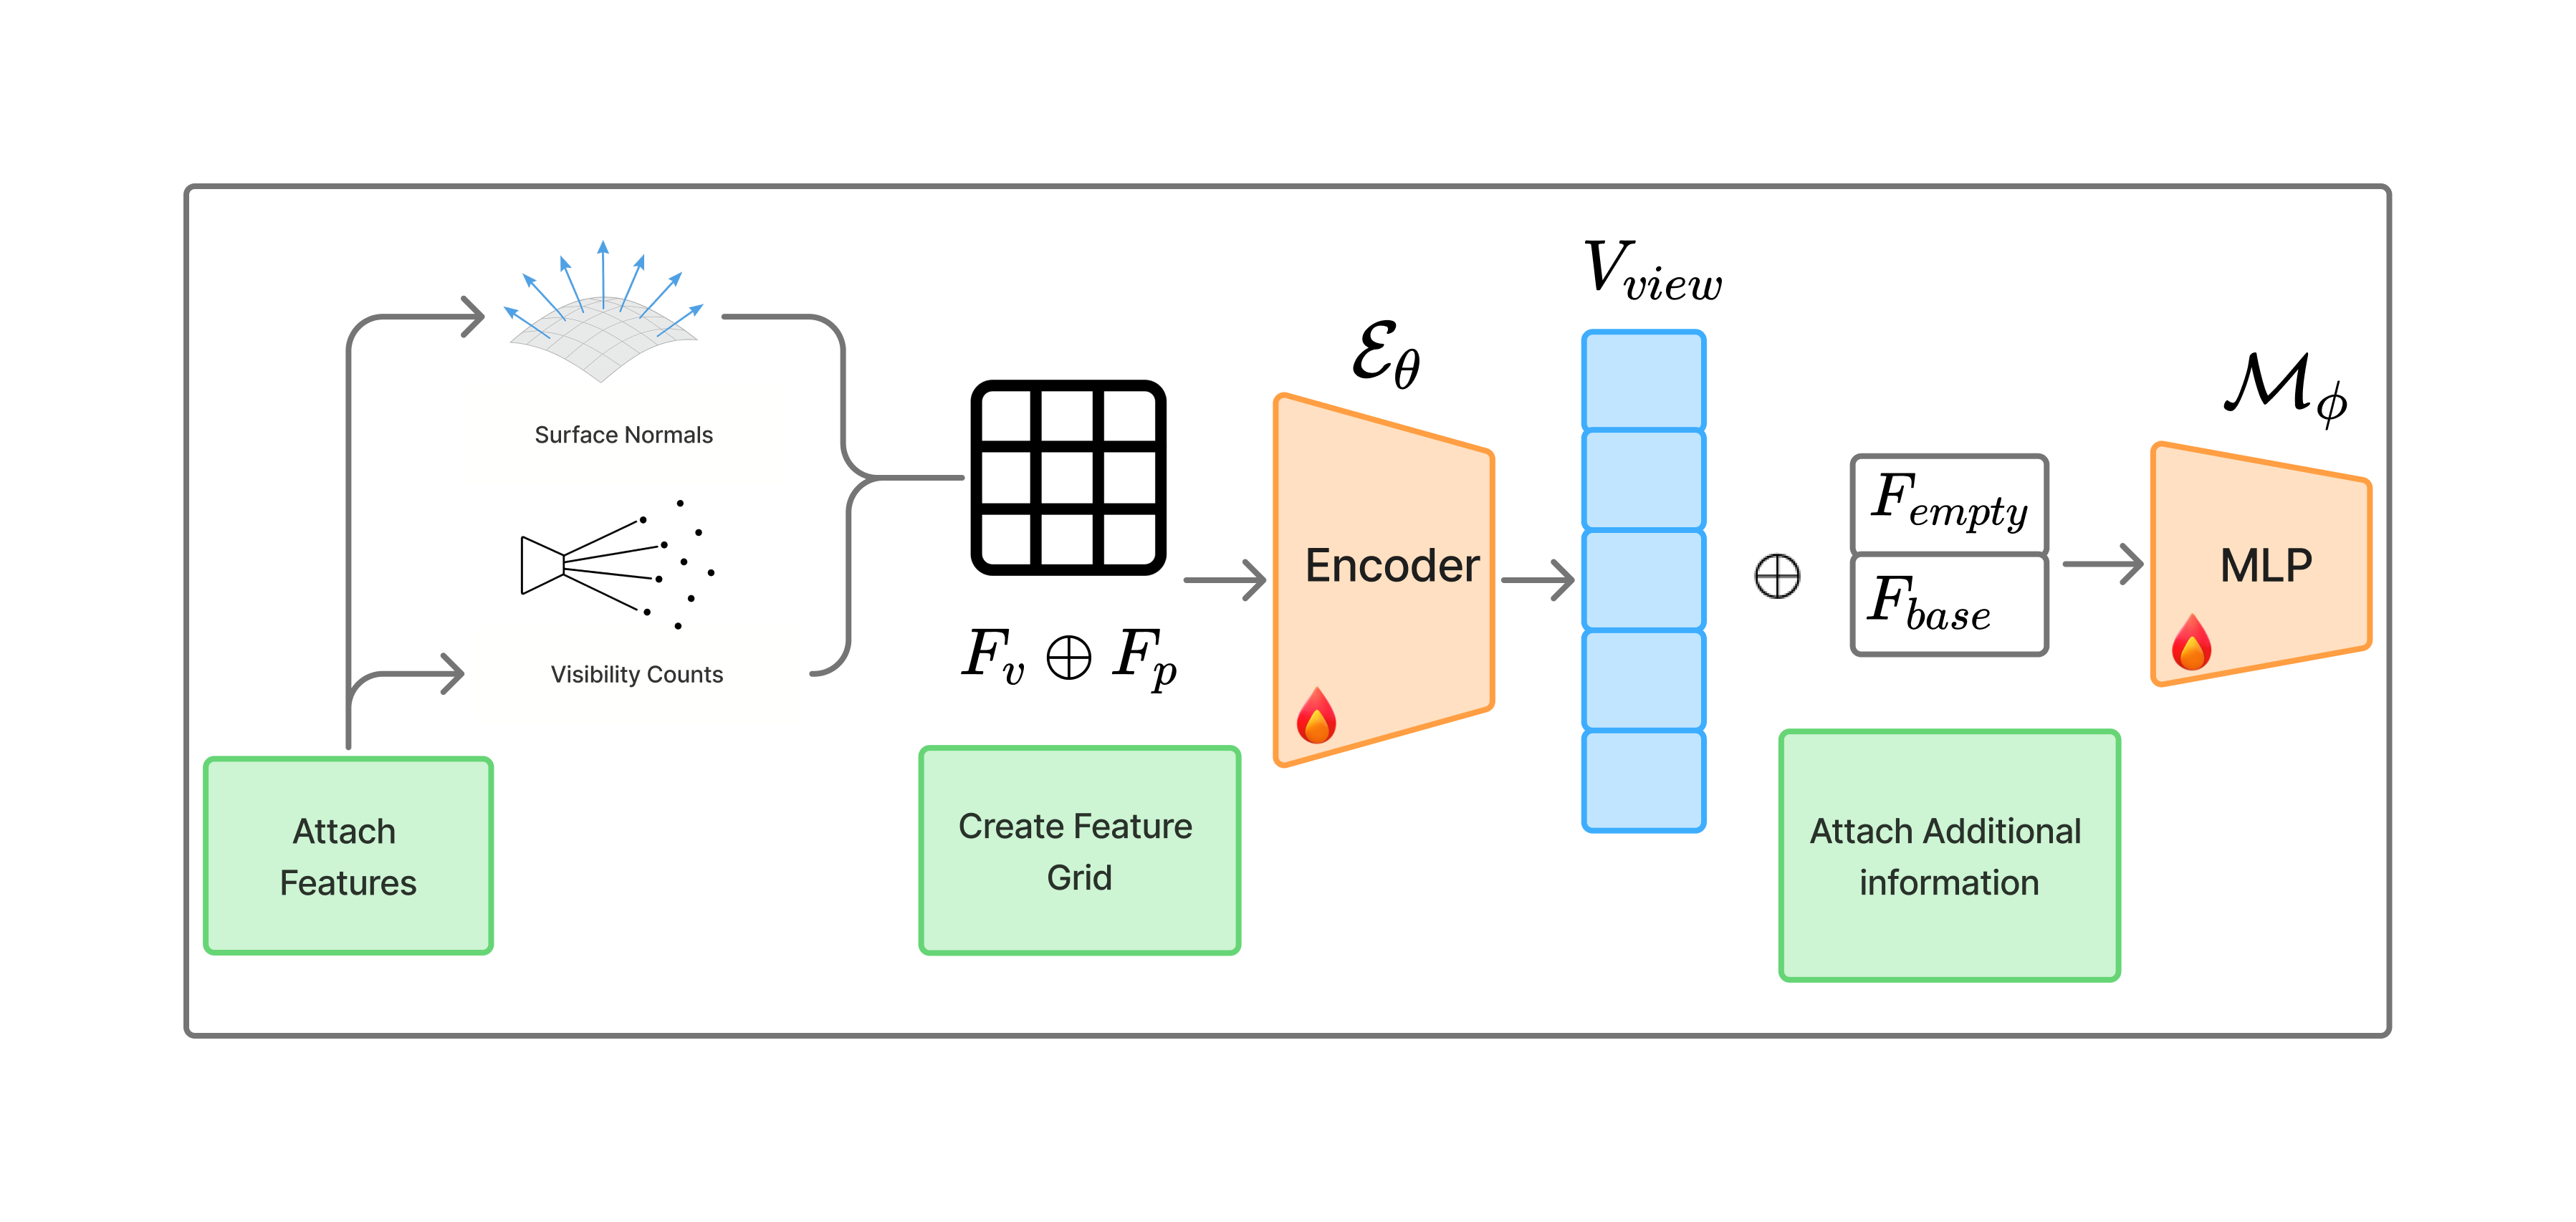
\includegraphics[width=\linewidth]{Figures/VIN_arch.png}
    \caption{VIN Architecture}
    \label{fig:arch_right}
  \end{subfigure}
  \vspace{-0.5em}
  \caption{
(a) VIN-NBV reconstructs the 3D scene from prior RGB-D captures, samples candidate viewpoints, and selects the one with the highest fitness predicted by the View Introspection Network (VIN) as the Next Best View (NBV), repeating until termination.
(b) VIN uses a 3D-aware featurization, including surface normals, visibility count, and coverage ($F_{empty}$), and is trained via imitation learning to predict fitness as the Relative Reconstruction Improvement over current observations.
}
  \label{fig:method_nbv_diagram}
  \vspace{-1.2em}
\end{figure*}

\section{Method}
\label{sec:method}
\vspace{-0.25em}

In the following section, we formalize the NBV problem and describe our VIN-NBV policy in detail.
We will first provide a mathematical overview of the NBV problem in Sec. \ref{ssec:prob}. Then, we will introduce our proposed sampling-based greedy NBV policy, VIN-NBV, in Sec. \ref{ssec:policy}, followed by the design of the View Introspection Network (VIN)  in \ref{ssec:vin_design} and its training in \ref{ssec:vin_training}.

\subsection{Problem Setup}
\label{ssec:prob}
\vspace{-0.25em}

Consider an agent that has acquired $k$ initial base images of a scene $I_{base}=\{I_{1},...,I_{k}\}$ from viewpoints with camera parameters $C_{base}=\{C_{1},...,C_{k}\}$ and depth maps $D_{base}=\{D_{1},...,D_{k}\}$ either captured with a depth sensor or predicted with a Monocular Depth Estimator or Multi-View Stereo algorithms. The agent then runs a 3D reconstruction pipeline using the initial base views to reconstruct the 3D scene as $\mathcal{R}_{base}$. The goal of NBV is to predict a set of $m$ next best views $C_{nbv}=\{C_{{1}},...,C_{m}\}$ from which the scene should be captured to maximize the reconstruction quality of the scene. 

More specifically, from $C_{nbv}$ we capture NBV images $I_{nbv}=\{I_{1},...,I_{m}\}$ and associated depth maps $D_{nbv}=\{D_{1},...,D_{m}\}$ and perform 3D reconstruction to create $\mathcal{R}_{final}$ using $I_{base} \cup I_{nbv}$ and $D_{base} \cup D_{nbv}$. While previous NBV techniques maximize coverage, we maximize reconstruction quality measured using the relative improvement of the Chamfer Distance of $\mathcal{R}_{final}$ over $\mathcal{R}_{base}$:
\begin{equation}
     C^{*}_{nbv} = \argmax_{C_{nbv}} ~\frac{CD(\mathcal{R}_{base},\mathcal{R}_{GT}) -CD(\mathcal{R}_{final},\mathcal{R}_{GT})}{CD(\mathcal{R}_{base},\mathcal{R}_{GT})},     
    \label{eq:cd-criteria}
\end{equation}

where $CD(\mathcal{R},\mathcal{R}_{GT})$ calculates the Chamfer Distance between the reconstructed point cloud of scene $\mathcal{R}$ and the ground-truth point cloud $\mathcal{R}_{GT}$.


\setlength{\intextsep}{0pt}
\setlength{\textfloatsep}{1pt}
\begin{algorithm}[!htb]
  \caption{VIN-NBV Policy}
  \label{method_nbv_algorithm}
  \begin{algorithmic}[1]
    \State $I^k_{\mathrm{base}}\gets\{I_1,\dots,I_k\}$
    \State $C^k_{\mathrm{base}}\gets\{C_1,\dots,C_k\}$
    \State $D^k_{\mathrm{base}}\gets\{D_1,\dots,D_k\}$
    \State $t = k$
    \While{not termination\_criteria()}
      \State Reconstruct $R^t_{\mathrm{base}}$ from $(I^t_{\mathrm{base}}, C^k_{\mathrm{base}}, D^k_{\mathrm{base}})$
      \State Sample a set of query views $\{q_i\}$
      \For{$i=1,\dots,n$}
        \State $\widehat{\mathcal{RRI}}(q_i) = \text{VIN}_\theta(R^{t}_{base}, C^t_{base}, C_{q_i})${\label{line:score_func}}
      \EndFor
        \State $C^t_*\gets\arg\max_q \mathcal{RRI}(q)$
        \State Capture (or render) $I^t_{*}$ and $D^{t}_{*}$ from $C^t_*$
        \State $I^{t+1}_{base} \leftarrow I^t_{base} \cup I^t_{*}$
        \State $D^{t+1}_{base} \leftarrow D^t_{base} \cup D^t_{*}$
        \State $C^{t+1}_{base} \leftarrow C^t_{base} \cup C^t_{*}$
        \State $t \mathrel{+}= 1$
    \EndWhile
    \State \Return $R_{\mathrm{final}}$
  \end{algorithmic}
\end{algorithm}

\vspace{0.5em}
\subsection{NBV Policy with View Introspection Network}
\label{ssec:policy}
\vspace{-0.25em}
We propose a simple greedy imitation learning based approach, where for each acquisition, the agent samples a set of query camera viewpoints and evaluates their fitness, and chooses the `best' one and repeats the process until some termination criterion has been reached. This acquisition policy has been described in Algorithm \ref{method_nbv_algorithm}.

The VIN-NBV policy begins with $I^k_{base}$, $C^k_{base}$, $D^k_{base}$ then iteratively selects next views until reaching a desired termination criteria, defined to fit downstream task constraints, e.g., number of image acquisitions, time traversed, battery life, etc. At each step, we update the reconstruction $R^t_{base}$ by back-projecting the RGB-D captures into 3D space. If only RGB images are available, we reconstruct $R^t_{base}$ using Multi-View Stereo or Monocular Depth Estimation. We then sample $n$ query views around this reconstruction to evaluate their fitness and choose the 'best'. 

Our key idea is the introduction of the View Introspection Network (VIN), which independently evaluates potential query views and predicts their fitness. Instead of evaluating the fitness of each view to maximize coverage, we focus on maximizing the reconstruction quality. More specifically, we define fitness criterion as the Relative Reconstruction Improvement ($\mathcal{RRI}$) over the base views by capturing the query view $q$ as defined in eq. \ref{eq:rri}. Relative Improvement is formulated to be independent of object types and scales, which otherwise affects the Chamfer Distance computation.

\vspace{-1em}
\begin{equation}
    \mathcal{RRI}(q_i) = \frac{CD(\mathcal{R}_{base},\mathcal{R}_{GT}) -CD(\mathcal{R}_{base \cup q_i},\mathcal{R}_{GT})}{CD(\mathcal{R}_{base},\mathcal{R}_{GT})}.
    \label{eq:rri}
\end{equation}

We train VIN to predict the RRI fitness criterion $\widehat{RRI}(q)$ for a query view $q$ by taking the existing reconstruction $R_{base}$, camera parameters $C_{base}$, and query view camera parameters $C_q$ as input:
\begin{equation}
    \widehat{\mathcal{RRI}}(q) = \text{VIN}_\theta(R_{base}, C_{base}, C_q).
\label{eq:vin}
\end{equation}
\vspace{-1.7em}

The design of VIN's neural architecture and its training are described in Sec \ref{ssec:vin_design} and \ref{ssec:vin_training}. After evaluating all $n$ query views, the VIN-NBV policy greedily selects the one with the highest improvement score. We move to the selected view position $C^t_*$ and acquire new RGB-D capture which we use to update $I^t_{base}$ $C^t_{base}$ $D^t_{base}$ to get $I^{t+1}_{base}$ $C^{t+1}_{base}$ $D^{t+1}_{base}$. Once we have reached our desired stopping criteria, we create and return our final 3D reconstruction $R_{final}$ using $I^{m}_{base}$ $C^{m}_{base}$ $D^{m}_{base}$.

Although we adopt a simple greedy acquisition strategy, our policy provides the flexibility to incorporate any desired constraints into the agent's acquisition strategy. In Section~\ref{sec:results}, we evaluate the VIN-NBV policy with constraints on the number of acquisitions and time in motion for the capture agent. Our method also allows the user to specify any sampling strategy to create a set of query views to evaluate, providing high adaptability to downstream applications.

\subsection{Design of VIN}\label{ssec:vin_design}
\vspace{-0.25em}

The View Introspection Network (VIN) estimates the utility of a candidate viewpoint by predicting its Relative Reconstruction Improvement (RRI) given the acquisition history and current reconstruction. There are three stages: first it reconstructs the scene, then it featurizes its geometry, and finally it encodes features to predict improvement.

From the current set of base RGB-D images $I_{base}$ and camera parameters $C_{base}$, we reconstruct a 3D point cloud $\mathcal{R}_{base}$. If a depth sensor is unavailable, monocular depth estimation or Multi-View Stereo can be substituted. Each point in $\mathcal{R}_{base}$ is enriched with surface normals, visibility count, and depth values. Surface normals estimate local geometry, with variance across neighboring points indicating complex surfaces that may require additional captures; low variance indicates planar regions that need less captures. Visibility count tracks the number of views from $I_{base}$ in which a point is observed. Points frequently seen in many views are less informative for new captures; points rarely seen may be more informative. Depth values provide distance information for projected pixels, helping to detect surface inconsistencies and missing regions.

For each candidate view $C_q$ the enriched point cloud is projected into its image plane, forming a feature grid (size 512$\times$512$\times$5). Here each pixel contains surface normals, visibility count, and depth after projection. We downsample this grid to 256$\times$256 via pooling to reduce computation and compute per-pixel variance to capture local geometric complexity. The down sampled feature grid is represented as $F_p$ and the per-pixel variances are $F_v$.

We also compute an empty feature $F_{empty}$ to provide explicit information about reconstruction coverage. This allows the VIN to focus on learning key information on top of coverage to predict reconstruction improvement. We consider a pixel to be "empty" if no point in $\mathcal{R}_{base}$ projects to it. We form a hull around non-empty pixels and count empty pixels inside and outside of the hull. Empty pixels inside the hull expose “holes” in the existing reconstruction and empty pixels outside the hull indicate potentially unseen geometry. We concatenate both of these values to create the two-element $F_{empty}$ feature vector. We use $F_{empty}$ as a lightweight proxy for more traditional reconstruction coverage measures.

To encode the features we define a convolutional encoder $V_{view} = \mathcal{E}_\theta\bigl(F_v \oplus F_p\bigr)$ that is applied to the feature grids and variances to transform the local per-pixel information into a global view feature vector $V_{view}$ of size $256\times1$, where $\oplus$ means concatenation. In addition to $V_{view}$, we also provide the number of base views $F_{base}$ to help indicate at what stage of the capture we are in; since helpful views in the earlier stages look different from helpful views in later stages, this may change how the model scores different views. We concatenate all of this information with $V_{view}$ and pass it through a MLP $\mathcal{M}(\cdot)$ to predict the final improvement score:

\vspace{-1.2em}
\begin{equation}
\widehat{\mathcal{RRI}}(q) = \mathcal{M}_\phi\bigl( \mathcal{E}_\theta\bigl(F_v \oplus F_p\bigr) \oplus F_{empty} \oplus F_{base}).
\end{equation}

\subsection{Training of VIN} \label{ssec:vin_training}
\vspace{-0.25em}

Our objective is to train the VIN to estimate the fitness of a query view, defined as its Relative Reconstruction Improvement ($\mathcal{RRI}(q)$) over the existing base views (as described in Equation \ref{eq:rri}). To achieve this, we adopt an imitation learning approach. For each object we sample and render a set of 120 RGB-D views that surround it, then at each step we
exhaustively compute the $\mathcal{RRI}$ for every query view. At each step we reconstruct the point cloud using the new image along with the previously captured base images. This computed score, which relies on access to the ground-truth 3D model and rendering engine, is referred to as the Oracle RRI. VIN is then trained to predict this Oracle RRI, without access to the rendered image, using only the RGB-D images from previously captured views and the camera parameters of the query view.

Directly regressing the $\mathcal{RRI}$ proves to be challenging. The model struggles to generalize across unseen objects and categories. To address this, we reformulate the task as a classification problem by discretizing the $\mathcal{RRI}$ into 15 ordinal classes, where class 0 indicates the least improvement and class 14 the highest. In this formulation, we recognize that misclassifications between distant classes are more detrimental than those between nearby ones. Therefore, even if VIN cannot always predict the optimal next-best view, it should still identify a reasonably good one. To enforce this, we use a ranking-aware classification loss: CORAL \cite{coral2020}. This loss transforms ordinal labels into a series of binary classification tasks, encouraging predictions that respect the natural order of the labels. This improves the model predictions and reduces large misclassifications.

An additional challenge arises in defining consistent class labels across different stages of acquisition. Early acquisitions often have higher $\mathcal{RRI}$ values because large portions of the scene remain unseen, so view selection has a greater impact. In contrast, later stages typically yield lower $\mathcal{RRI}$ values, as improvements become more incremental, focusing on resolving occlusions and small gaps. Using a fixed class assignment strategy across all stages would misclassify even the best views in later stages as lower-quality.

To overcome this, we normalize $\mathcal{RRI}$ values in a stage-independent manner. We group our training data by capture stage, defined by the number of base views, and determine the standard deviation and mean of the $\mathcal{RRI}$ values in these groups. We then take $\mathcal{RRI}$ for each query view and convert it into a z-score based on the number of standard deviations they are from the mean of their group. We soft-clip the z-scores using a tanh function, to prevent extreme outliers, and then group views into 15 dynamically sized bins, ensuring a similar number of samples in each bin. We use these bins as our final class labels.